\chapter{Примеры решения задач}
\section{Пример I}

\subsection{Постановка задачи}
\renewcommand{\labelenumi}{\arabic{enumi})}
Задана ЗЛП с целевой функцией:
\begin{equation}
	F(\vec{X}) = x_1+x_2 \to max.
\end{equation}

Система ограничений имеет следующий вид:
\begin{equation}
\label{system}
\begin{cases}
20x_1+10x_2 \le 45\\
2x_1+7x_2 \le 14\\
x_i \ge 0 \\
\end{cases}
\end{equation}.

Необходимо:
\begin{enumerate}
\item Решить исходную ЗЛП симплекс-методом;
\item Решить исходную ЗЛП графически;
\item Из последней симплекс-таблицы найти решение исходной и двойственной задач;
\item Построить двойственную ЗЛП;
\item Решить двойственную ЗЛП методом искусственного базиса;
\item Решить двойственную ЗЛП графически;
\item Из последней симплекс-таблицы найти решение исходной и двойственной задач;
\item Сравнить результаты.
\end{enumerate}

\subsection{Решение исходной ЗЛП симплекс-методом}
Введем балансовые переменные и приведем к каноническому виду.
Для нахождения максимума, умножим целевую функцию на -1.

$$-F(\vec{X}) = -(-x_1-x_2) \to max$$
\begin{equation}
\label{cannonical}
\begin{cases}
20x_1+10x_2+x_3=45\\
2x_1+7x_2+x_4=14\\
x_i, s_i \ge 0 \\
\end{cases}
\end{equation}

Составим таблицу и решим задачу симплекс-методом.

\begin{center}
\begin{tabular*}{\textwidth}{@{\extracolsep{\fill}}|c|c|c|c|c|c|c|c|c|}
\hline
$i$ & Базис & $C_i$ & B & $C_1 = -1$ & $C_2 = -1$ & $C_3 = 0$ & $C_4 = 0$ & $\Theta_i$ \\
\hline
$1$ & $P_3$ & $0$ & $45$ & $20$ & $10$ & $1$ & $0$ & $2,25$\\
$2$ & $P_4$ & $0$ & $14$ & $2$ & $7$ & $0$ & $1$ & $7$\\
\hline
$m+1$ & ~ & ~ & $0$ & $1$ & $1$ & $0$ & $0$ & ~ \\
\hline
\end{tabular*}
\end{center}
\begin{center}
\begin{tabular*}{\textwidth}{@{\extracolsep{\fill}}|c|c|c|c|c|c|c|c|c|}
\hline
$i$ & Базис & $C_i$ & B & $C_1 = -1$ & $C_2 = -1$ & $C_3 = 0$ & $C_4 = 0$ & $\Theta_i$ \\
\hline
$1$ & $P_1$ & $-1$ & $2,25$ & $1$ & $0,5$ & $0,05$ & $0$ & $4,5$\\
$2$ & $P_4$ & $0$ & $9,5$ & $0$ & $6$ & $-0,1$ & $1$ & $1,583$\\
\hline
$m+1$ & ~ & ~ & $-2,25$ & $0$ & $0,5$ & $-0,05$ & $0$ & ~ \\
\hline
\end{tabular*}
\end{center}
\begin{center}
\begin{tabular*}{\textwidth}{@{\extracolsep{\fill}}|c|c|c|c|c|c|c|c|c|}
\hline
$i$ & Базис & $C_i$ & B & $C_1 = -1$ & $C_2 = -1$ & $C_3 = 0$ & $C_4 = 0$ & $\Theta_i$ \\
\hline
$1$ & $P_1$ & $-1$ & $1,458$ & $1$ & $0$ & $0,05833$ & $-0,08333$ & $4,5$\\
$2$ & $P_2$ & $-1$ & $1,583$ & $0$ & $1$ & $-0,01667$ & $0,1667$ & $1,583$\\
\hline
$m+1$ & ~ & ~ & $-3,042$ & $0$ & $0$ & $-0,04167$ & $-0,08333$ & ~ \\
$m+1$ & ~ & ~ & $3,042$ & $0$ & $0$ & $0,04167$ & $0,08333$ & ~ \\
\hline
\end{tabular*}
\end{center}
Получен оптимальный план: $X^{опт} = (1,458;1,583)$, и оптимальное значение целевой функции $F^{опт} = 3,04$.

\subsection{Решение исходной ЗЛП графическим методом}
\begin{figure}[ht]
\centering
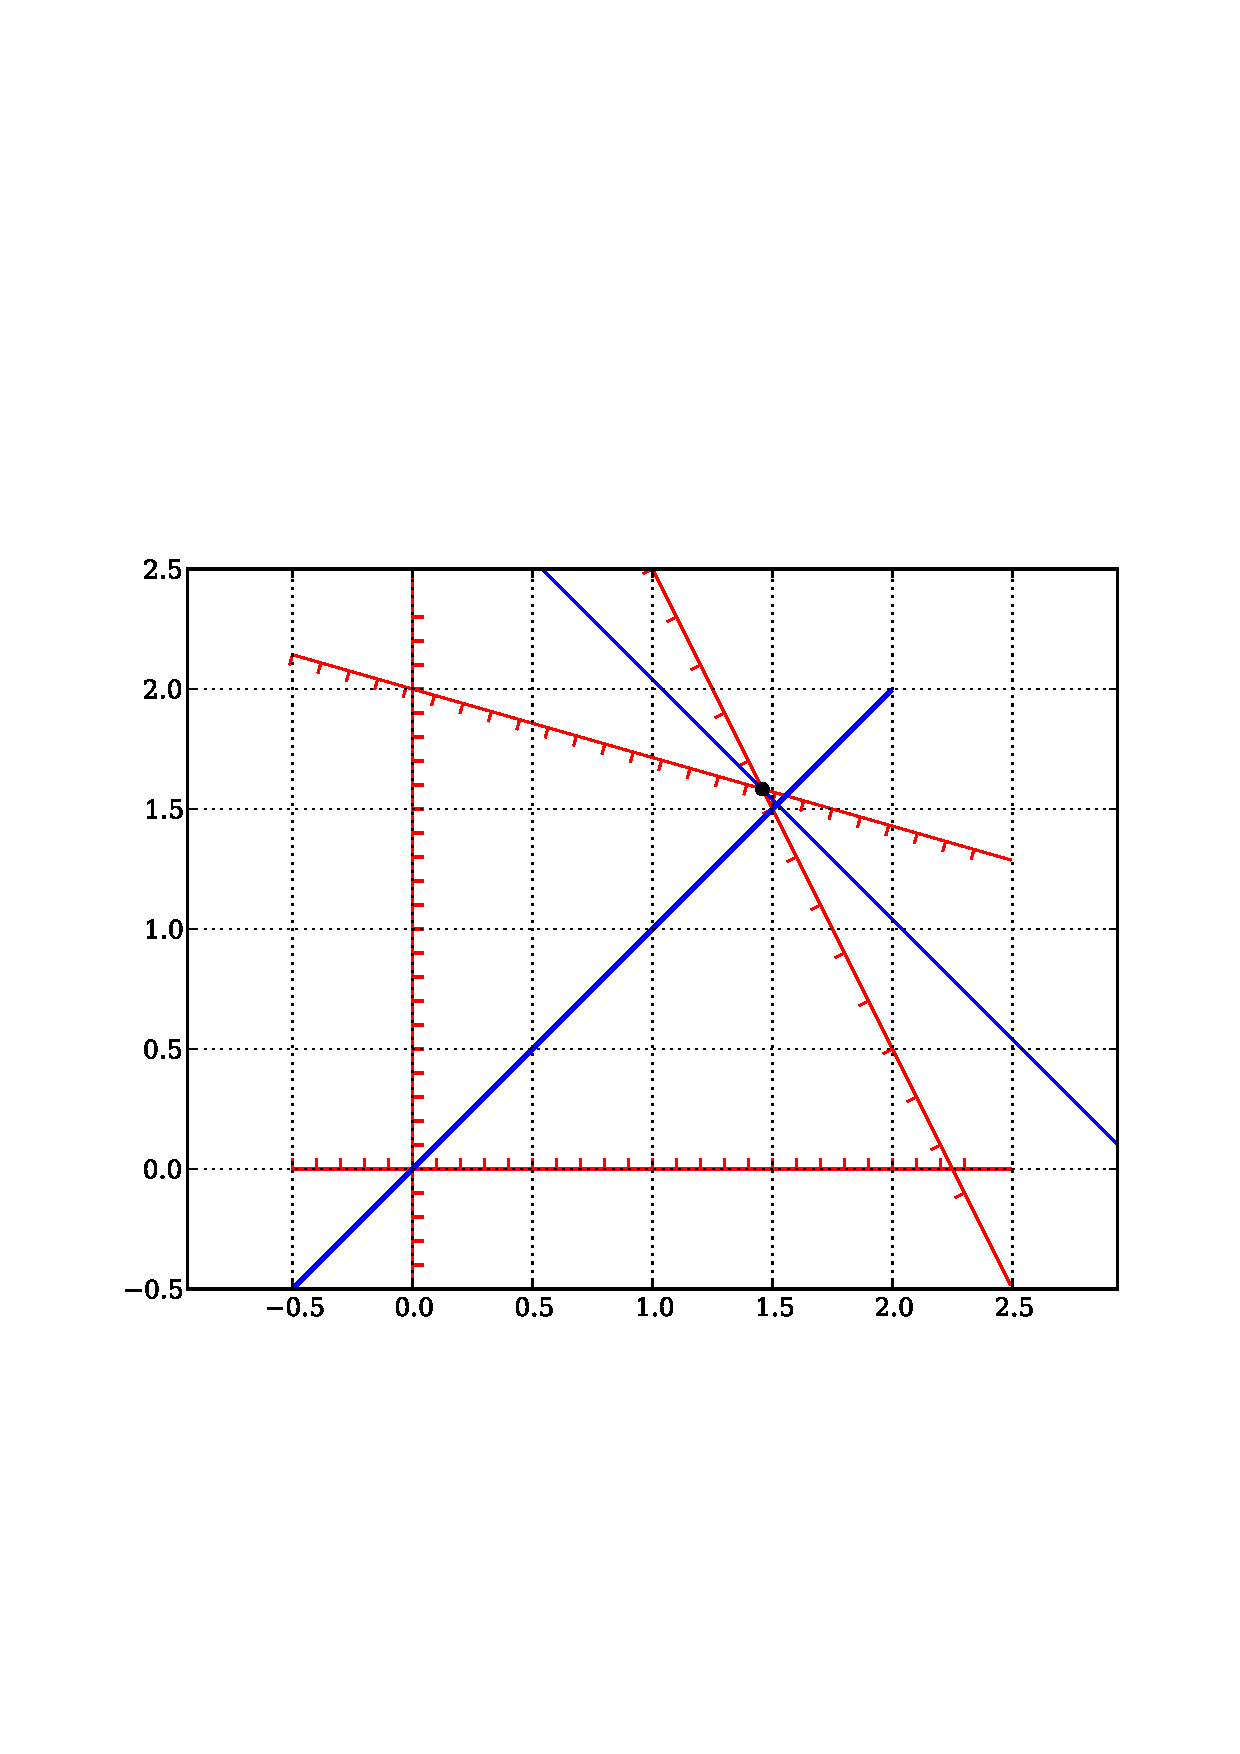
\includegraphics[width=\textwidth]{img/11}
\caption{Решение графическим методом}\label{11}
\end{figure}

\subsection{Решение исходной и двойственной ЗЛП из симплекс-таблицы}
Для исходной ЗЛП был получен оптимальный план и оптимальное решение:
\begin{align*}
	X^{опт} = (1,458;1,583),&~ F^{опт} = 3,04.
\end{align*}


Тогда оптимальный план и значение двойственной симметричной ЗЛП:
\begin{align*}
	Y^{опт} = (0,042; 0,083),&~ Z^{опт} = 3,04.
\end{align*}

\subsection{Построение двойственной ЗЛП}
Построим двойственную симметричную ЗЛП:

\begin{equation}
	Z(\vec{Y}) = 45 y_1 + 14y_2 \to min,
\end{equation}

\begin{equation}
\label{system}
\begin{cases}
20y_1 + 2y_2 \ge 1, \\
10y_1 + 7y_2 \ge 1, \\
y_1, y_2 \ge 0. \\
\end{cases}
\end{equation}

\subsection{Решение двойственной ЗЛП методом искусственного базиса}
Введем искусственные переменные и приведем к каноническому виду.
\begin{equation}
	Z(\vec{Y}) = 45y_1+14y_2+Wy_5+Wy_6 \to min
\end{equation}

\begin{equation}
\label{cannonical}
\begin{cases}
20y_1+2y_2-y_3+ s_5=1\\
10y_1+7y_2-y_4+ s_6=1\\
y_i, s_i \ge 0 \\
\end{cases}
\end{equation}
\begin{center}
\begin{tabular*}{\textwidth}{@{\extracolsep{\fill}}|c|c|c|c|c|c|c|c|c|c|c|}
\hline
$i$ & Базис & $B_i$ & C & $B_1 = 45$ & $B_2 = 14$ & $B_3 = 0$ & $B_4 = 0$ & $B_5 = W$ & $B_6 = W$ & $\Theta_i$ \\
\hline
$1$ & $P_5$ & W & $1$ & $20$ & $2$ & $-1$ & $0$ & $1$ & $0$ & $0,05$\\
$2$ & $P_6$ & W & $1$ & $10$ & $7$ & $0$ & $-1$ & $0$ & $1$ & $0,1$\\
\hline
$m+1$ & ~ & ~ & $0$ & $-45$ & $-14$ & $0$ & $0$ & $0$ & $0$ & ~ \\
\hline
$m+2$ & ~ & ~ & $2W$ & $30W$ & $9W$ & $-1W$ & $-1W$ & $0W$ & $0W$ & ~ \\
\hline
\end{tabular*}
\end{center}
\begin{center}
\begin{tabular*}{\textwidth}{@{\extracolsep{\fill}}|c|c|c|c|c|c|c|c|c|c|c|}
\hline
$i$ & Базис & $B_i$ & C & $B_1 = 45$ & $B_2 = 14$ & $B_3 = 0$ & $B_4 = 0$ & $B_5 = W$ & $B_6 = W$ & $\Theta_i$ \\
\hline
$1$ & $P_1$ & $45$ & $0,05$ & $1$ & $0,1$ & $-0,05$ & $0$ & $0,05$ & $0$ & $0,5$\\
$2$ & $P_6$ & W & $0,5$ & $0$ & $6$ & $0,5$ & $-1$ & $-0,5$ & $1$ & $0,08333$\\
\hline
$m+1$ & ~ & ~ & $2,25$ & $0$ & $-9,5$ & $-2,25$ & $0$ & $2,25$ & $0$ & ~ \\
\hline
$m+2$ & ~ & ~ & $0,5W$ & $0W$ & $6W$ & $0,5W$ & $-1W$ & $-1,5W$ & $0W$ & ~ \\
\hline
\end{tabular*}
\end{center}
\begin{center}
\begin{tabular*}{\textwidth}{@{\extracolsep{\fill}}|c|c|c|c|c|c|c|c|c|c|c|}
\hline
$i$ & Базис & $B_i$ & C & $B_1 = 45$ & $B_2 = 14$ & $B_3 = 0$ & $B_4 = 0$ & $B_5 = W$ & $B_6 = W$ & $\Theta_i$ \\
\hline
$1$ & $P_1$ & $45$ & $0,04167$ & $1$ & $0$ & $-0,05833$ & $0,01667$ & $0,05833$ & $-0,01667$ & ~\\
$2$ & $P_2$ & $14$ & $0,08333$ & $0$ & $1$ & $0,08333$ & $-0,1667$ & $-0,08333$ & $0,1667$ & ~\\
\hline
~ & ~ & ~ & $3,042$ & $0$ & $0$ & $-1,458$ & $-1,583$ & $1,458$ & $1,583$ & ~ \\
\hline
~ & ~ & ~ & $0W$ & $0W$ & $0W$ & $0W$ & $0W$ & $-1W$ & $-1W$ & ~ \\
\hline
\end{tabular*}
\end{center}
Получен оптимальный план: $Y^{опт} = (0,0417;0,0833)$, и оптимальное значение целевой функции $Z^{опт} = 3,04$.

\subsection{Решение двойственной ЗЛП графическим методом}
\begin{figure}[ht]
\centering
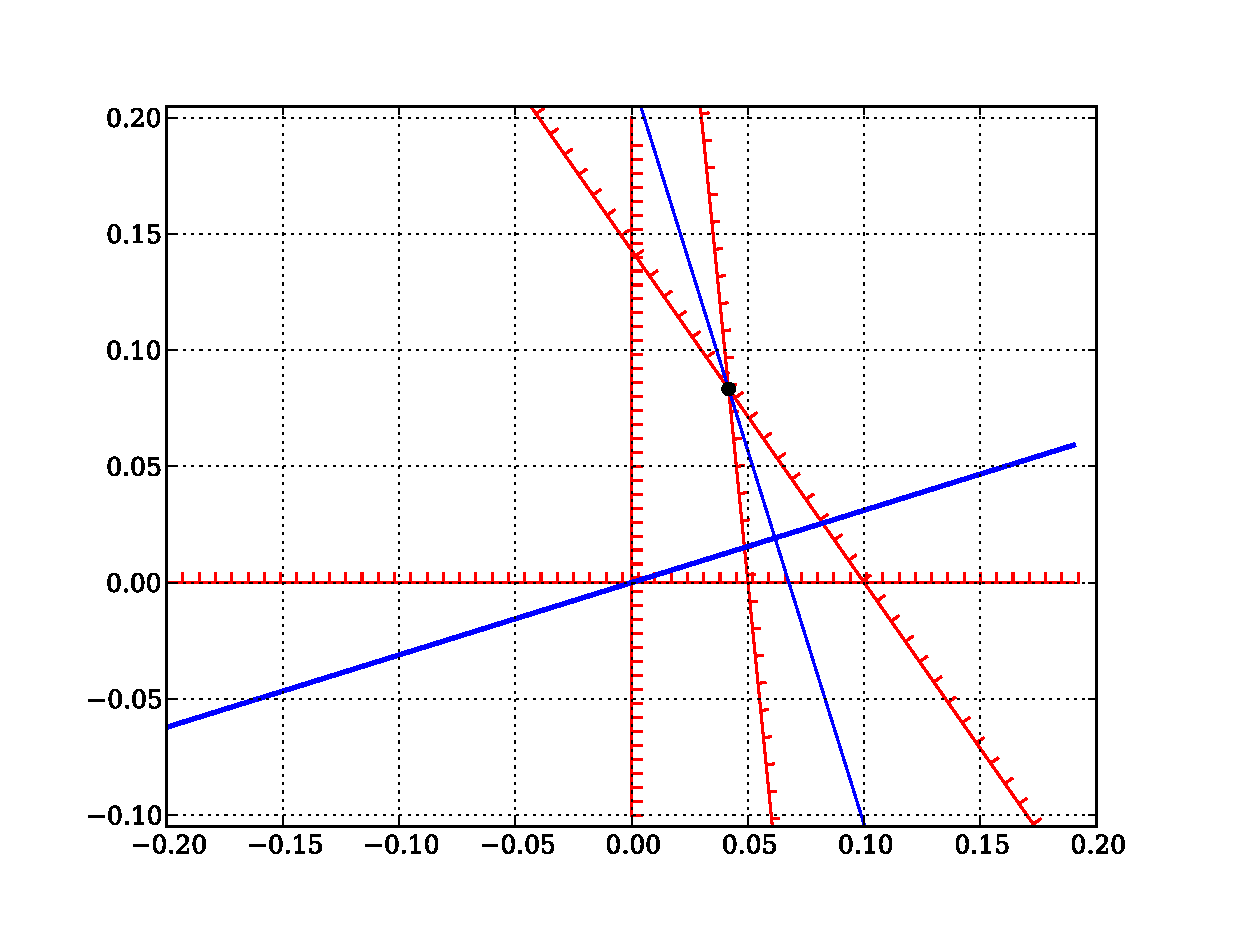
\includegraphics[width=\textwidth]{img/12}
\caption{Решение графическим методом}\label{11}
\end{figure}

\subsection{Решение исходной и двойственной ЗЛП из симплекс-таблицы}
Для двойственной ЗЛП был получен оптимальный план и оптимальное решение:
\begin{align*}
	Y^{опт} = (0,042; 0,084),&~ Z^{опт} = 3,04.
\end{align*}

Тогда оптимальный план и значение исходной ЗЛП:
\begin{align*}
	X^{опт} = (1,458;1,583),&~ F^{опт} = 3,04.
\end{align*}

\subsection{Сравнение результатов}
Из результатов видно, что $max F = min Z$ в независимости от порядка и способа
вычисления, что подтверждает правильность выполнения
основной теоремы двойственности в данном примере.